\documentclass[../main.tex]{subfiles}

\begin{document}

    \begin{itemize}
        \item \textbf{Kaskadowe arkusze stylów} (ang. Cascading Style Sheets) - język opisu sposoby prezentacji (wyglądu) dokumentu HTML.
        \item CSS umożliwia rozdzielenie struktury i zawartości dokumentu od sposobu jego prezentacji\\

        \item Określanie czcionek (rodziny, koloru, wielkości, pugrubienia, itp)
        \item Określenie marginesów, odstępów między liniami
        \item Określenie rozmiarów i położenia poszczególnych elementów strony
        \item Określanie obramowań i wypełnień
        \item Zmiana spsobu prezentacji standardowych elementów (np. punktory w listach)
    \end{itemize}


    \subsubsection{Selektory}




    \begin{itemize}
        \item Selektor decyduje do którego elementu strony są stosowane właściwości
        \item Kryterium wyboru może być m.in. typ elementu, atrybuty (w szczególności id i class) oraz położenie elementu względem innych elementów.
        \item Pseduo-elementy dają dostęp m.in. do fragmentów elementów (::first-letter)
        \item Można także używać pseudo-klas dających dostęp do informacji nie zawartych bezpośrednio w dkoumencie (:hover, :visited)
    \end{itemize}


    \begin{table}[H]
        \begin{center}
            \begin{tabular}{|p{4cm}|p{4cm}|p{4cm}|p{4cm}|}
                \hline
                \textbf{Content-Type} & text/html & text/html & application/xhtml+xml\\
                \hline
                \textbf{doctype} & brak/stary & poprawny & bez znaczenia\\
                \hline
                \textbf{Wynik} & HTML(quirks mode) & HTML 4.01 / HTML 5 & XHTML\\
                \hline
            \end{tabular}
        \end{center}
    \end{table}
    W przypadku trybu html nie zauważy np. zamknięcia elementu typu <strong />.

    Np: .class, \#id, $*$, element, (element,element), (element element), [attribute=value].

    \textbf{Priorytety}
    \begin{table}[H]
        \begin{center}
            \begin{tabular}{|p{2cm}|p{4cm}|p{8cm}|}
                \hline
                \textbf{Priority} & \textbf{CSS source type} & \textbf{Description}\\
                \hline
                \hline
                1 & Importance & The !important annotation overwrites the previous priority types\\
                \hline
                2 & Inline & A style applied to an HTML element via HTML 'style' attribute\\
                \hline
                3 & Media Type & A property definition applies to all media types, unless a media specific CSS is defined\\
                \hline
                4 & User defined & Most browsers have the accessibility feature: a user defined CSS\\
                \hline
                5 & Selector specificity & A specific contextual selector (\#heading p) overwrites generic definition\\
                \hline
                6 & Rule order & Last rule declaration has a higher priority\\
                \hline
                7 & Parent inheritance & If a property is not specified, it is inherited from a parent element\\
                \hline
                8 & CSS property definition in HTML document & CSS rule or CSS inline style overwrites a default browser value\\
                \hline
                9 & Browser default & The lowest priority: browser default value is determined by W3C initial value specifications\\
                \hline
            \end{tabular}
        \end{center}
    \end{table}
    Style związane z fontami (tekstem) sa dziedziczone z elementu rodzica. Większość pozostałych stylów nie jest dziedziczona.

    \textbf{Specyficzność.}\\

    Specyficzność określa "szczegółowość" selektora:
    \begin{itemize}
        \item prosty selektor (selektor elementu) ma specyficzność (p) = 0, 0 , 0, 1
        \item selektor klasy ma specyficzność (.head-button)= 0, 0 , 1, 0
        \item selektor oparty na id ma specyficzność (\#save-button) = 0, 1 , 0, 0
        \item style inline (umieszczony w elemencie) ma specyficzność = 1, 0 , 0, 0
    \end{itemize}
    Selector "body \#content .data img:hover" ma specyficzność równą 0,1,2,2.


    \subsection{Box Model}

    \begin{table}[H]
        \begin{center}
            \begin{tabular}{p{8cm} p{8cm}}
                \begin{itemize}
                    \item Każdy element HTML można traktować jako prostokąt. Zawartość elementu (content) jest otoczona wypełnieniem (padding), obramowaniem (border) oraz marginesem (margin).
                    \item W zależności od wartości box-sizing (content-box lub border-box) obliczany jest całkowity rozmiar elementu.
                \end{itemize}
                &
                \raisebox{-\totalheight}{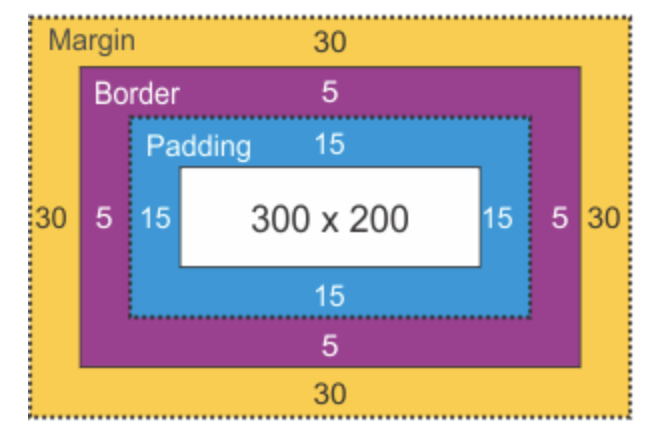
\includegraphics[width=8cm]{boxmodel.png}}
                \\
            \end{tabular}
        \end{center}
    \end{table}

    \subsection{Dodatki}
    \begin{itemize}
        \item \textbf{CSS Transforms} - pozwala na transformacje takie jak przesunięcie, skalowanie, obracanie, itp.
        \begin{itemize}
            \item translate()
            \item rotate()
            \item scale()
            \item skewX()
            \item skewY()
            \item matrix()
        \end{itemize}

        \item \textbf{CSS Transitions} - pozwala na płynną zmianę wartości.

        \item \textbf{SS Flexbox Layout}
        \begin{itemize}
            \item Elastyczny menadżer układu elementów na stronie.
            \item Elementy mogą być typu flex-container i/lub flex-item
            \item Dla \textbf{flex-container} możemy określić kierunek i sposób ulożenia elementów flex-item (pionowo/poziomo, prawo/lewo, zawijanie wierszy, wykorzystanie wolnej przestrzeni)
            \item Dla \textbf{flex-item} możemy okreslić zdolnośc elementu do powiększania/zmniejszania, wpełania pustej przestrzeni (także w stosunku do sąsiednich elementów), bazowy rozmiar, kolejność wyświetlania, itp.
            \item Przy pomocy Flexboxa stosunkowo łatwo wykonac podział strony na kilka kolumn tej samej wysokości.
        \end{itemize}
    \end{itemize}
\end{document}